\documentclass{ximera}

\title{3D Coordinate Changes}
\author{Zack Reed}

\begin{document}
\begin{abstract}
In this activity we apply cylindrical and spherical coordinate systems to compute masses of 3D objects with variable density, seeing how choosing the right coordinates reduces complicated nested bounds to simple constants.
\end{abstract}
\maketitle


\section*{Application: Mass of 3D Objects}

While you've already seen cylindrical coordiantes (polar + height), we'll also introduce spherical coordinates, which better handle rotations in 3D space generally.

\begin{problem}
Below are two figures of 3D shapes that can be efficiently described with respect to cylindrical and spherical coordinates.

First, cylindrical coordinates are given as

\begin{align*}
x &= r\cos\theta \\
y &= r\sin\theta \\
z &= z
\end{align*}

Spherical coordinates are given as

\begin{align*}
x &= \rho\sin\phi\cos\theta \\
y &= \rho\sin\phi\sin\theta \\
z &= \rho\cos\phi
\end{align*}

As before, $\theta$ is rotation around the vertical axis. For spherical coordinates, we also include $\phi$, which is rotation downward from the vertical axis.

\begin{center}
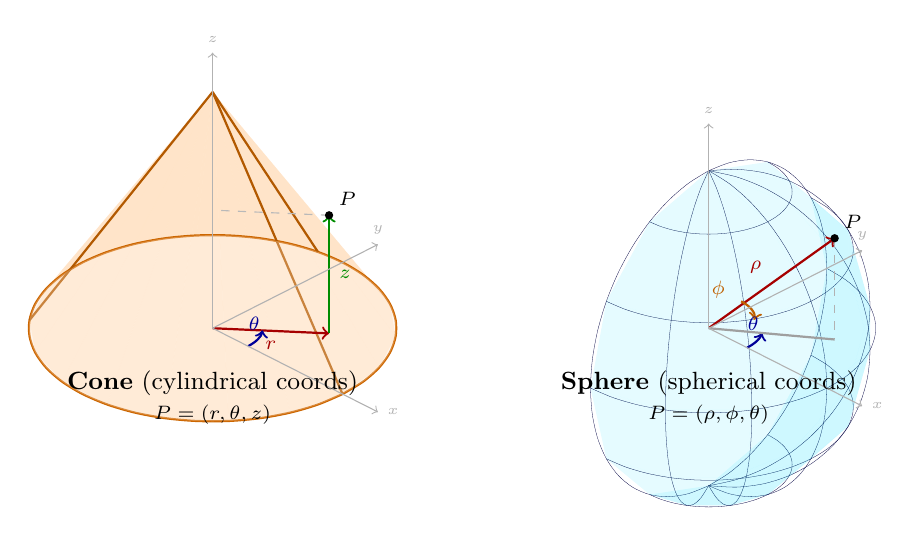
\begin{tikzpicture}[scale=1.0]

%=== LEFT: Cone in 3D — show a point P located by (r, theta, z) ===
\begin{scope}[x={(0.75cm,-0.38cm)}, y={(0.75cm,0.38cm)}, z={(0cm,1.0cm)}, xshift=0.5cm]
  % Cone: tip at z=5 (top), base radius=4 at z=0. Scale 1m -> 0.55cm.
  % Draw cone surface (orange)
  \foreach \th in {0,20,...,340} {
    \pgfmathsetmacro{\thn}{\th+20}
    \fill[orange!30!white,opacity=0.45]
      (0,0,3) -- ({2.2*cos(\th)},{2.2*sin(\th)},0)
             -- ({2.2*cos(\thn)},{2.2*sin(\thn)},0) -- cycle;
  }
  % Base circle and outline
  \draw[orange!80!black,thick,domain=0:360,samples=37,smooth,variable=\t]
    plot ({2.2*cos(\t)},{2.2*sin(\t)},0);
  \draw[orange!70!black,thick] (0,0,3) -- (2.2,0,0);
  \draw[orange!70!black,thick] (0,0,3) -- ({2.2*cos(100)},{2.2*sin(100)},0);
  \draw[orange!70!black,thick] (0,0,3) -- ({2.2*cos(220)},{2.2*sin(220)},0);
  \fill[orange!20,opacity=0.3,domain=0:360,samples=37,smooth,variable=\t]
    plot ({2.2*cos(\t)},{2.2*sin(\t)},0) -- cycle;

  % A sample point P at (r=1.4, theta=40deg, z=1.5)
  \def\pr{1.4} \def\pth{40} \def\pz{1.5}
  \pgfmathsetmacro{\px}{\pr*cos(\pth)}
  \pgfmathsetmacro{\py}{\pr*sin(\pth)}

  % Dashed construction lines
  \draw[gray!55,dashed,thin] (\px,\py,0) -- (\px,\py,\pz);   % vertical up to P
  \draw[gray!55,dashed,thin] (0,0,0) -- (\px,\py,0);          % radial on base
  \draw[gray!55,dashed,thin] (\px,\py,\pz) -- (0,0,\pz);      % horizontal to z-axis

  % r arrow (radial on base plane)
  \draw[->,red!65!black,thick] (0,0,0) -- (\px,\py,0)
    node[midway,below,font=\scriptsize,red!65!black]{$r$};

  % theta arc on base plane
  \draw[->,blue!60!black,thick]
    ({0.6*cos(0)},{0.6*sin(0)},0)
    arc[start angle=0,end angle=\pth,radius=0.6];
  \node[blue!60!black,font=\scriptsize] at ({0.55*cos(20)},{0.55*sin(20)},0.18) {$\theta$};

  % z arrow (vertical)
  \draw[->,green!55!black,thick] (\px,\py,0) -- (\px,\py,\pz)
    node[midway,right,font=\scriptsize,green!55!black]{$z$};

  % Point P
  \fill[black] (\px,\py,\pz) circle (1.5pt);
  \node[font=\scriptsize,above right] at (\px,\py,\pz) {$P$};

  % Axes
  \draw[->,gray!60,thin] (0,0,0) -- (2.8,0,0) node[right,font=\tiny]{$x$};
  \draw[->,gray!60,thin] (0,0,0) -- (0,2.8,0) node[above,font=\tiny]{$y$};
  \draw[->,gray!60,thin] (0,0,0) -- (0,0,3.5) node[above,font=\tiny]{$z$};

  \node[font=\small,align=center] at (0,0,-0.7) {\textbf{Cone} (cylindrical coords)};
  \node[font=\scriptsize,align=center] at (0,0,-1.1) {$P=(r,\theta,z)$};
\end{scope}

%=== RIGHT: Sphere in 3D — show a point P located by (rho, phi, theta) ===
\begin{scope}[x={(0.75cm,-0.38cm)}, y={(0.75cm,0.38cm)}, z={(0cm,1.0cm)}, xshift=6.8cm]
  % Sphere wireframe, radius=2
  \def\RS{2.0}
  % Lat lines (front half) — ultra-thin, recessive
  \foreach \ph in {30,60,90,120,150} {
    \pgfmathsetmacro{\rr}{\RS*sin(\ph)} \pgfmathsetmacro{\zz}{\RS*cos(\ph)}
    \draw[blue!25!black,ultra thin,domain=-90:90,smooth,samples=19,variable=\t]
      plot ({\rr*cos(\t)},{\rr*sin(\t)},\zz);
  }
  % Long lines (front half) — ultra-thin, recessive
  \foreach \th in {-90,-60,...,90} {
    \draw[blue!25!black,ultra thin,domain=0:180,smooth,samples=19,variable=\p]
      plot ({\RS*sin(\p)*cos(\th)},{\RS*sin(\p)*sin(\th)},{\RS*cos(\p)});
  }
  % Light fill, front hemisphere
  \foreach \ph in {0,30,...,150} {
    \pgfmathsetmacro{\phn}{\ph+30}
    \pgfmathsetmacro{\ra}{\RS*sin(\ph)} \pgfmathsetmacro{\za}{\RS*cos(\ph)}
    \pgfmathsetmacro{\rb}{\RS*sin(\phn)} \pgfmathsetmacro{\zb}{\RS*cos(\phn)}
    \foreach \th in {-90,-60,...,60} {
      \pgfmathsetmacro{\thn}{\th+30}
      \fill[blue!15!cyan,opacity=0.10]
        ({\ra*cos(\th)},{\ra*sin(\th)},\za)
        -- ({\rb*cos(\th)},{\rb*sin(\th)},\zb)
        -- ({\rb*cos(\thn)},{\rb*sin(\thn)},\zb)
        -- ({\ra*cos(\thn)},{\ra*sin(\thn)},\za) -- cycle;
    }
  }

  % Sample point P at (rho=RS, phi=50, theta=35)
  \def\pphi{50} \def\pth{35}
  \pgfmathsetmacro{\px}{\RS*sin(\pphi)*cos(\pth)}
  \pgfmathsetmacro{\py}{\RS*sin(\pphi)*sin(\pth)}
  \pgfmathsetmacro{\pz}{\RS*cos(\pphi)}
  \pgfmathsetmacro{\pxf}{\RS*sin(\pphi)*cos(0)}  % phi plane foot on xz

  % rho vector from origin to P (surface)
  \draw[->,red!65!black,thick] (0,0,0) -- (\px,\py,\pz)
    node[midway,above left,font=\scriptsize,red!65!black]{$\rho$};

  % phi angle arc in meridian plane (theta=pth)
  % arc from z-axis to line toward P, in the x-z plane projected
  \draw[orange!75!black,thick,->]
    ({0.55*cos(0)},{0.55*sin(0)},{\RS*0.55/\RS})
    arc[start angle=90, delta angle={-\pphi}, radius=0.55];
  \node[orange!75!black,font=\scriptsize] at ({0.28*sin(\pphi/2)*cos(\pth)},{0.28*sin(\pphi/2)*sin(\pth)},{0.55*cos(\pphi/2)}) {$\phi$};

  % theta arc on equatorial plane
  \draw[blue!60!black,thick,->]
    ({0.65*cos(0)},{0.65*sin(0)},0)
    arc[start angle=0,end angle=\pth,radius=0.65];
  \node[blue!60!black,font=\scriptsize] at ({0.6*cos(\pth/2)},{0.6*sin(\pth/2)},0.2) {$\theta$};

  % Construction lines: base radial on equatorial plane (solid/prominent) + height drop (dashed)
  \pgfmathsetmacro{\pxeq}{\RS*sin(\pphi)*cos(\pth)}
  \pgfmathsetmacro{\pyeq}{\RS*sin(\pphi)*sin(\pth)}
  \draw[gray!60,dashed,semithick] (\px,\py,\pz) -- (\pxeq,\pyeq,0);
  \draw[gray!75,thick] (0,0,0) -- (\pxeq,\pyeq,0);

  % Point P
  \fill[black] (\px,\py,\pz) circle (1.5pt);
  \node[font=\scriptsize,above right] at (\px,\py,\pz) {$P$};

  % Axes
  \draw[->,gray!60,thin] (0,0,0) -- (2.6,0,0) node[right,font=\tiny]{$x$};
  \draw[->,gray!60,thin] (0,0,0) -- (0,2.6,0) node[above,font=\tiny]{$y$};
  \draw[->,gray!60,thin] (0,0,0) -- (0,0,2.6) node[above,font=\tiny]{$z$};

  \node[font=\small,align=center] at (0,0,-0.7) {\textbf{Sphere} (spherical coords)};
  \node[font=\scriptsize,align=center] at (0,0,-1.1) {$P=(\rho,\phi,\theta)$};
\end{scope}

\end{tikzpicture}
\end{center}

For the cone, which coordinate system is most natural?
\begin{multipleChoice}
    \choice{Rectangular $(x,y,z)$}
    \choice[correct]{Cylindrical $(r,\theta,z)$}
    \choice{Spherical $(\rho,\phi,\theta)$}
\end{multipleChoice}

For the sphere, which coordinate system is most natural?
\begin{multipleChoice}
    \choice{Rectangular $(x,y,z)$}
    \choice{Cylindrical $(r,\theta,z)$}
    \choice[correct]{Spherical $(\rho,\phi,\theta)$}
\end{multipleChoice}

\end{problem}

\section*{Cylindrical Coordinates}

We've already set up the important geometry shift in the last module, shifting from $dx\,dy$ to $r\,dr\,d\theta$ in the $xy$-plane. Now we also have to include the vertical dimension $z$, so the volume element becomes $dV = r\,dr\,d\theta\,dz$.

\begin{definition}
\textbf{Cylindrical coordinates} $(r, \theta, z)$ extend polar coordinates into 3D:
\begin{itemize}
    \item $x = r\cos\theta$
    \item $y = r\sin\theta$
    \item $z = z$
\end{itemize}

The volume element is: $dV = r\,dr\,d\theta\,dz$
\end{definition}

The following diagram re-emphasizes the basic idea of the coordinate system change, but includes a small $z$-change for the small cylindrical height.

\begin{center}
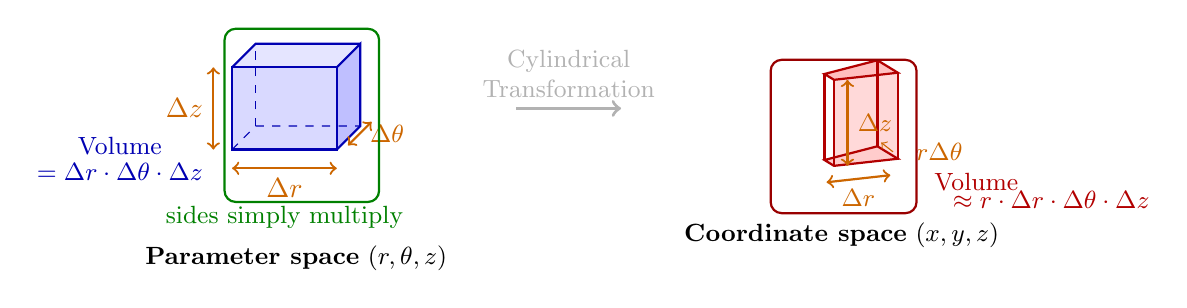
\begin{tikzpicture}[scale=0.95]

%=== LEFT: parameter space (r, theta, z) rectangular box ===
\begin{scope}[xshift=0cm]
  % Draw as a simple 3D oblique box
  % using a pseudo-3D projection: x-axis goes right, y-axis goes up, z-axis goes upper-right
  % basis: e_r = (1,0), e_theta = (0,1), e_z = (0.45, 0.45)
  \def\er{(1,0)}  \def\et{(0,1)}  \def\ez{(0.45,0.45)}
  \def\W{1.4}  \def\H{1.1}  \def\D{0.7}
  % The eight corners (origin + combinations)
  % O = (0,0), A=W*er, B=H*et, C=D*ez, AB=A+B, AC=A+C, BC=B+C, ABC=A+B+C
  \coordinate (O) at (0,0);
  \coordinate (A) at (\W,0);
  \coordinate (B) at (0,\H);
  \coordinate (C) at ({\D*0.45},{\D*0.45});
  \coordinate (AB) at (\W,\H);
  \coordinate (AC) at ({\W+\D*0.45},{\D*0.45});
  \coordinate (BC) at ({\D*0.45},{\H+\D*0.45});
  \coordinate (ABC) at ({\W+\D*0.45},{\H+\D*0.45});

  % Fill faces
  \fill[blue!15] (O)--(A)--(AB)--(B)--cycle;
  \fill[blue!25] (A)--(AC)--(ABC)--(AB)--cycle;
  \fill[blue!10] (B)--(AB)--(ABC)--(BC)--cycle;

  % Draw edges
  \draw[blue!70!black,thick] (O)--(A)--(AB)--(B)--cycle;
  \draw[blue!70!black,thick] (A)--(AC)--(ABC)--(AB);
  \draw[blue!70!black,thick] (B)--(BC)--(ABC);
  \draw[blue!70!black,dashed] (O)--(C)--(AC);
  \draw[blue!70!black,dashed] (C)--(BC);

  % Dimension labels
  \draw[<->,orange!80!black,thick] (0,-0.25)--(\W,-0.25) node[midway,below]{$\Delta r$};
  \draw[<->,orange!80!black,thick] (-0.25,0)--(-0.25,\H) node[midway,left]{$\Delta z$};
  \draw[<->,orange!80!black,thick] ({\W+0.15},{0.08*\D})--({\W+\D*0.45+0.15},{\D*0.45+0.08*\D})
        node[midway,right,font=\small]{$\Delta\theta$};

  % Volume annotation
  \node[blue!70!black,font=\small,align=center] at ({-1.5},{\H/2-.5}) {Volume};
  \node[blue!70!black,font=\small,align=center] at ({-1.5},{-0.3}) {$= \Delta r\cdot\Delta\theta\cdot\Delta z$};

  \draw[green!50!black,rounded corners,thick] (-.1,-.7) rectangle ({\W+\D*0.45+0.25},{\H+\D*0.45+0.2});
  \node[green!50!black,font=\small] at ({\W/2},-0.9) {sides simply multiply};
  \node[font=\small,align=center,below] at ({(\W+\D*0.45)/2},-1.15)
        {\textbf{Parameter space} $(r,\theta,z)$};
\end{scope}

%=== ARROW ===
\begin{scope}[xshift=3.8cm]
  \draw[->,very thick,gray!60](0,0.55)--(1.4,0.55)
    node[midway,above,align=center,font=\small]{Cylindrical\\Transformation};

%=== RIGHT: coordinate space (x,y,z) curved prism ===
\begin{scope}[xshift=3.5cm, yshift=-0.3cm]
  % Draw using standard 3D oblique: x goes right, y goes upper-right, z goes up
  % A curved prism: bottom face is a polar wedge, extruded up by Delta z
  % r_in=0.7, r_out=1.5, theta_a=25, theta_b=55, z_bot=0, z_top=1.1
  \def\rI{0.7}  \def\rO{1.5}  \def\thA{25}  \def\thB{55}  \def\zt{1.15}
  % Project 3D (x,y,z) -> 2D: px = x + 0.4*y, py = z + 0.25*y
  % bottom face corners: 4 points at z=0
  % IL = inner-left, IR = inner-right, OL = outer-left, OR = outer-right
  \pgfmathsetmacro{\ILx}{\rI*cos(\thA)}  \pgfmathsetmacro{\ILy}{\rI*sin(\thA)}
  \pgfmathsetmacro{\IRx}{\rI*cos(\thB)}  \pgfmathsetmacro{\IRy}{\rI*sin(\thB)}
  \pgfmathsetmacro{\OLx}{\rO*cos(\thA)}  \pgfmathsetmacro{\OLy}{\rO*sin(\thA)}
  \pgfmathsetmacro{\ORx}{\rO*cos(\thB)}  \pgfmathsetmacro{\ORy}{\rO*sin(\thB)}
  % 2D projected coords (px, py) = (x + 0.38*y, 0 + 0.28*y) for z=0
  % and (x + 0.38*y, zt + 0.28*y) for z=zt
  \pgfmathsetmacro{\pILx}{\ILx+0.38*\ILy}  \pgfmathsetmacro{\pILy}{0.28*\ILy}
  \pgfmathsetmacro{\pIRx}{\IRx+0.38*\IRy}  \pgfmathsetmacro{\pIRy}{0.28*\IRy}
  \pgfmathsetmacro{\pOLx}{\OLx+0.38*\OLy}  \pgfmathsetmacro{\pOLy}{0.28*\OLy}
  \pgfmathsetmacro{\pORx}{\ORx+0.38*\ORy}  \pgfmathsetmacro{\pORy}{0.28*\ORy}
  % Top versions (add zt to z component -> add zt to py)
  \pgfmathsetmacro{\tILy}{\pILy+\zt}  \pgfmathsetmacro{\tIRy}{\pIRy+\zt}
  \pgfmathsetmacro{\tOLy}{\pOLy+\zt}  \pgfmathsetmacro{\tORy}{\pORy+\zt}

  % Back face (for visibility order)
  \fill[red!10]
    (\pOLx,\pOLy) -- (\pORx,\pORy) -- (\pORx,\tORy) -- (\pOLx,\tOLy) -- cycle;
  \fill[red!15]
    (\pILx,\pILy) -- (\pOLx,\pOLy) -- (\pOLx,\tOLy) -- (\pILx,\tILy) -- cycle;

  % Bottom curved face (approximate with straight lines)
  \fill[red!20]
    (\pILx,\pILy) -- (\pOLx,\pOLy) -- (\pORx,\pORy) -- (\pIRx,\pIRy) -- cycle;

  % Top curved face
  \fill[red!25]
    (\pILx,\tILy) -- (\pOLx,\tOLy) -- (\pORx,\tORy) -- (\pIRx,\tIRy) -- cycle;

  % Draw all edges
  \draw[red!70!black,thick]
    (\pILx,\pILy) -- (\pOLx,\pOLy) -- (\pORx,\pORy) -- (\pIRx,\pIRy) -- cycle;
  \draw[red!70!black,thick]
    (\pILx,\tILy) -- (\pOLx,\tOLy) -- (\pORx,\tORy) -- (\pIRx,\tIRy) -- cycle;
  \draw[red!70!black,thick] (\pILx,\pILy)--(\pILx,\tILy);
  \draw[red!70!black,thick] (\pIRx,\pIRy)--(\pIRx,\tIRy);
  \draw[red!70!black,thick] (\pOLx,\pOLy)--(\pOLx,\tOLy);
  \draw[red!70!black,thick] (\pORx,\pORy)--(\pORx,\tORy);

  % Dimension labels
  \pgfmathsetmacro{\rmid}{(\rI+\rO)/2}
  \pgfmathsetmacro{\tmid}{(\thA+\thB)/2}
  \pgfmathsetmacro{\pmx}{\rmid*cos(\thA)+0.38*\rmid*sin(\thA)}
  \pgfmathsetmacro{\pmy}{0.28*\rmid*sin(\thA)}
  \draw[<->,orange!80!black,thick]
    ({\pILx-0.1},{\pILy-0.22}) -- ({\pOLx-0.1},{\pOLy-0.22})
    node[midway,below,font=\small]{$\Delta r$};

  % arc label
  \pgfmathsetmacro{\pARCx}{\rO*cos(\tmid)+0.38*\rO*sin(\tmid)+0.2}
  \pgfmathsetmacro{\pARCy}{0.28*\rO*sin(\tmid)}
  \node[orange!80!black,right,font=\small] at (\pARCx,\pARCy) {$r\Delta\theta$};
  \draw[orange!80!black,->,thin] (\pARCx-0.18,\pARCy) -- (\pORx+0.05,\pORy+0.05);

  % height label
  \draw[<->,orange!80!black,thick]
    ({\pILx+0.18},{\pILy}) -- ({\pILx+0.18},{\tILy})
    node[midway,right,font=\small]{$\Delta z$};

  % Bounding box (tight around prism only, mirroring green box on left)
  \draw[red!60!black,rounded corners,thick] (-0.1,-0.55) rectangle (1.85,{\zt+0.35});
  \node[font=\small,align=center,below] at (0.85,{-0.55})
        {\textbf{Coordinate space} $(x,y,z)$};

  % Volume annotation to the RIGHT (mirroring left side)
  \node[red!70!black,font=\small,align=center] at (2.65,{\zt/2-.7}) {Volume};
  \node[red!70!black,font=\small,align=center] at (3.65,{\zt/2-.95}) {$\approx r\cdot\Delta r\cdot\Delta\theta\cdot\Delta z$};
\end{scope}

\end{scope}

\end{tikzpicture}
\end{center}

The parameter-space box has sides $\Delta r$, $\Delta\theta$, $\Delta z$ --- we'd naively compute $\Delta r \cdot \Delta\theta \cdot \Delta z$.  

But in cylindrical coordinates the angular side becomes an \emph{arc} of length $r\,\Delta\theta$, so the linear approximation of the prism's volume is $r\,\Delta r\,\Delta\theta\,\Delta z$.  As the cell shrinks, we treat the arc as straight and get exactly $dV = r\,dr\,d\theta\,dz$.

\begin{problem}
Cylindrical coordinates are built from:
\begin{selectAll}
    \choice[correct]{Polar coordinates $(r,\theta)$ in the $xy$-plane}
    \choice[correct]{Height $z$ perpendicular to the plane}
    \choice{Spherical shells}
    \choice[correct]{The familiar extra factor of $r$ from polar integrals}
\end{selectAll}

The volume element $dV = r\,dr\,d\theta\,dz$ comes from:
\begin{multipleChoice}
    \choice{Multiplying all three differentials}
    \choice[correct]{Taking a polar area element $dA = r\,dr\,d\theta$ and extending it by height $dz$}
    \choice{Spherical geometry}
\end{multipleChoice}
\end{problem}

\begin{problem}
Explore cylindrical coordinates visually.

\begin{expandable}{stuff}{GeoGebra Instructions}
    Select ``Show Cylinder'' view. Use sliders to change $r$, $\theta$, and $z$. Click ``Zoom to Volume Element'' to see the small piece $dV = r\,dr\,d\theta\,dz$.
\end{expandable}

\begin{center}
\geogebra{xqrs44yg}{750}{675}
\end{center}

As you vary $r$, $\theta$, $z$, observe:
\begin{selectAll}
    \choice[correct]{$r$ controls distance from the $z$-axis}
    \choice[correct]{$\theta$ controls rotation around the $z$-axis}
    \choice[correct]{$z$ controls height}
    \choice{The volume element shape is always a cube}
\end{selectAll}


\end{problem}

Before going through some examples, here is a quick video visualizing the main intuitions behind cylindrical coordinates and the volume element $dV = r\,dr\,d\theta\,dz$:


\youtube{4FutuyIc7e8}



\textbf{Mass of Fluid in a Rotating Container}

A cylindrical container (radius 2 m, height 5 m) rotates, causing the fluid density to vary:
$$\delta(r,z) = 1000 + 50r^2 - 20z \text{ kg/m}^3$$

where $(r, \theta, z)$ are cylindrical coordinates.


\begin{center}
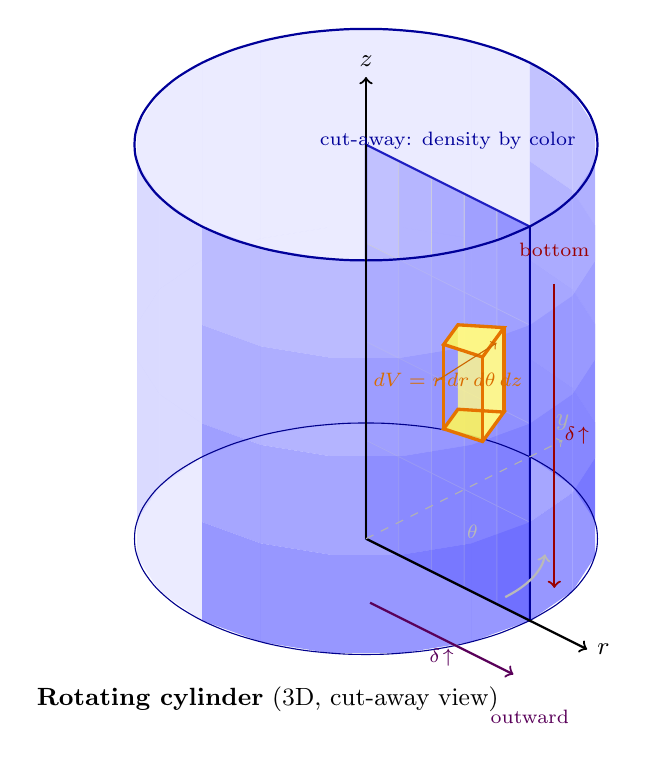
\begin{tikzpicture}[x={(0.8cm,-0.4cm)}, y={(0.8cm,0.4cm)}, z={(0cm,1.1cm)}, scale=1.3]
% 3D rotating cylinder: radius R=2, height H=3.5
% Density increases with r (centrifugal) and decreases with z (pressure)
\def\RR{2.0}
\def\HH{3.5}

% --- Interior r-z cross-section at theta=0 (cut-away face, shows both gradients) ---
\foreach \ri in {0,0.4,...,1.6} {
  \foreach \zb in {0,0.875,...,2.625} {
    \pgfmathsetmacro{\zn}{\zb+0.875}
    \pgfmathsetmacro{\rn}{\ri+0.4}
    % denser at large r AND at small z
    \pgfmathtruncatemacro{\bright}{20 + 30*\ri/2 + 15*(1 - \zb/3.5)}
    \fill[blue!\bright!white,opacity=0.88]
      (\ri,0,\zb) -- (\ri,0,\zn) -- (\rn,0,\zn) -- (\rn,0,\zb) -- cycle;
    \draw[gray!30,very thin]
      (\ri,0,\zb) -- (\ri,0,\zn) -- (\rn,0,\zn) -- (\rn,0,\zb) -- cycle;
  }
}
% Cross-section border
\draw[blue!70!black,thick] (0,0,0) -- (\RR,0,0) -- (\RR,0,\HH) -- (0,0,\HH) -- cycle;

% --- Back half outer surface (theta 90..270, translucent) ---
\foreach \za/\zb in {0/1.75, 1.75/3.5} {
  \foreach \ta in {90,108,...,252} {
    \pgfmathsetmacro{\tbn}{\ta+18}
    \fill[blue!40!white,opacity=0.20]
      ({\RR*cos(\ta)},{\RR*sin(\ta)},\za)
      -- ({\RR*cos(\ta)},{\RR*sin(\ta)},\zb)
      -- ({\RR*cos(\tbn)},{\RR*sin(\tbn)},\zb)
      -- ({\RR*cos(\tbn)},{\RR*sin(\tbn)},\za) -- cycle;
  }
}

% --- Front half outer surface (theta -90..90), z-banded for z-density gradient ---
\foreach \za/\zb/\bright in {0/0.875/58, 0.875/1.75/50, 1.75/2.625/42, 2.625/3.5/34} {
  \foreach \ta in {-90,-72,...,72} {
    \pgfmathsetmacro{\tbn}{\ta+18}
    \fill[blue!\bright!white,opacity=0.70]
      ({\RR*cos(\ta)},{\RR*sin(\ta)},\za)
      -- ({\RR*cos(\ta)},{\RR*sin(\ta)},\zb)
      -- ({\RR*cos(\tbn)},{\RR*sin(\tbn)},\zb)
      -- ({\RR*cos(\tbn)},{\RR*sin(\tbn)},\za) -- cycle;
  }
}

% Top and bottom ellipses
\draw[blue!60!black,thick,domain=0:360,smooth,samples=37,variable=\t]
  plot ({\RR*cos(\t)},{\RR*sin(\t)},\HH);
\draw[blue!55!black,thin,domain=0:360,smooth,samples=37,variable=\t]
  plot ({\RR*cos(\t)},{\RR*sin(\t)},0);
\draw[blue!60!black,thick] (\RR,0,0) -- (\RR,0,\HH);

% Axes
\draw[->,thick] (0,0,0) -- ({\RR+0.7},0,0) node[right,font=\small]{$r$};
\draw[->,thick] (0,0,0) -- (0,0,{\HH+0.6}) node[above,font=\small]{$z$};
\draw[->,dashed,gray!60] (0,0,0) -- (0,{\RR+0.4},0) node[above,font=\small]{$y$};

% theta sweep arrow
\draw[->,thick,gray!55] ({0.85*\RR},0,0.1) arc[start angle=0,end angle=40,radius={0.85*\RR*0.7}];
\node[font=\scriptsize,gray!55] at (0.7,0.6,0.1) {$\theta$};

% --- Highlighted dV wedge element ---
\def\rI{0.8} \def\rO{1.2}
\def\taA{12} \def\taB{38}
\def\zlo{1.2} \def\zhi{1.95}

\fill[yellow!65,opacity=0.88]
  ({\rI*cos(\taA)},{\rI*sin(\taA)},\zlo)
  -- ({\rI*cos(\taB)},{\rI*sin(\taB)},\zlo)
  -- ({\rO*cos(\taB)},{\rO*sin(\taB)},\zlo)
  -- ({\rO*cos(\taA)},{\rO*sin(\taA)},\zlo) -- cycle;
\fill[yellow!65,opacity=0.88]
  ({\rI*cos(\taA)},{\rI*sin(\taA)},\zhi)
  -- ({\rI*cos(\taB)},{\rI*sin(\taB)},\zhi)
  -- ({\rO*cos(\taB)},{\rO*sin(\taB)},\zhi)
  -- ({\rO*cos(\taA)},{\rO*sin(\taA)},\zhi) -- cycle;
\fill[yellow!45,opacity=0.82]
  ({\rO*cos(\taA)},{\rO*sin(\taA)},\zlo) -- ({\rO*cos(\taA)},{\rO*sin(\taA)},\zhi)
  -- ({\rO*cos(\taB)},{\rO*sin(\taB)},\zhi) -- ({\rO*cos(\taB)},{\rO*sin(\taB)},\zlo) -- cycle;
\fill[yellow!45,opacity=0.82]
  ({\rI*cos(\taB)},{\rI*sin(\taB)},\zlo) -- ({\rI*cos(\taB)},{\rI*sin(\taB)},\zhi)
  -- ({\rO*cos(\taB)},{\rO*sin(\taB)},\zhi) -- ({\rO*cos(\taB)},{\rO*sin(\taB)},\zlo) -- cycle;
\draw[orange!90!black,very thick]
  ({\rI*cos(\taA)},{\rI*sin(\taA)},\zlo)
  -- ({\rI*cos(\taB)},{\rI*sin(\taB)},\zlo)
  -- ({\rO*cos(\taB)},{\rO*sin(\taB)},\zlo)
  -- ({\rO*cos(\taA)},{\rO*sin(\taA)},\zlo) -- cycle;
\draw[orange!90!black,very thick]
  ({\rI*cos(\taA)},{\rI*sin(\taA)},\zhi)
  -- ({\rI*cos(\taB)},{\rI*sin(\taB)},\zhi)
  -- ({\rO*cos(\taB)},{\rO*sin(\taB)},\zhi)
  -- ({\rO*cos(\taA)},{\rO*sin(\taA)},\zhi) -- cycle;
\draw[orange!90!black,very thick]
  ({\rI*cos(\taA)},{\rI*sin(\taA)},\zlo) -- ({\rI*cos(\taA)},{\rI*sin(\taA)},\zhi);
\draw[orange!90!black,very thick]
  ({\rO*cos(\taA)},{\rO*sin(\taA)},\zlo) -- ({\rO*cos(\taA)},{\rO*sin(\taA)},\zhi);
\draw[orange!90!black,very thick]
  ({\rO*cos(\taB)},{\rO*sin(\taB)},\zlo) -- ({\rO*cos(\taB)},{\rO*sin(\taB)},\zhi);

% dV label
\node[font=\scriptsize,orange!85!black,align=center] at (2.0,-1.0,2.5)
  {$dV=r\,dr\,d\theta\,dz$};
\draw[orange!80!black,->,thin]
  (1.6,-0.75,2.25) -- ({\rO*cos(25)},{\rO*sin(25)},{\zhi});

% Density arrows
\draw[->,thick,red!60!black] ({\RR+0.3},0,3.1) -- ({\RR+0.3},0,0.4)
  node[midway,right,font=\scriptsize]{$\delta\!\uparrow$};
\draw[->,thick,violet!70!black] (0.05,0,-0.55) -- (1.8,0,-0.55)
  node[midway,below,font=\scriptsize]{$\delta\!\uparrow$};
\node[font=\scriptsize,red!60!black] at ({\RR+0.3},0,3.4) {bottom};
\node[font=\scriptsize,violet!70!black] at (2.0,0,-0.85) {outward};
\node[font=\scriptsize,blue!60!black,align=center] at ({0.5*\RR},0,{\HH+0.4})
  {cut-away: density by color};

\node[font=\small,align=center] at (0.4,-1.6,-0.7)
  {\textbf{Rotating cylinder} (3D, cut-away view)};
\end{tikzpicture}
\end{center}


In cylindrical coordinates, the volume element is:
$$dV = \answer{r}\,dr\,d\theta\,dz$$

\begin{problem}


The small mass element: $dM = \delta(r,z) \cdot dV = \answer{(1000 + 50r^2 - 20z) \cdot r}\,dr\,d\theta\,dz$

The integral setup for total mass:
$$M = \int_{\answer{0}}^{\answer{2\pi}} \int_{\answer{0}}^{\answer{5}} \int_{\answer{0}}^{\answer{2}} (1000 + 50r^2 - 20z) \cdot r\,dr\,dz\,d\theta$$

Notice the density:
\begin{selectAll}
    \choice[correct]{Increases with distance from the axis (centrifugal effect)}
    \choice[correct]{Decreases with height (pressure effect)}
    \choice{Depends on angle $\theta$}
    \choice[correct]{Is independent of angle (axial symmetry)}
\end{selectAll}


\end{problem}

Now let's do a problem where the solid doesn't exactly match the coordinate system.

\begin{problem}

\textbf{Part A: Finding Mass}

Consider the following cone of height $H=5$ m and base radius $R=4$ m, with density $\delta = 3 + 2z$ (where $z$ is height from tip):

\begin{center}
\begin{tikzpicture}[scale=0.9]
  % Cone cross-section showing r_max at each height
  % Tip at top (0,3), base at bottom (-2.4,0),(2.4,0)
  \shade[top color=blue!10, bottom color=blue!50, opacity=0.75]
    (0,3) -- (-2.4,0) -- (2.4,0) -- cycle;
  \draw[black,thick] (0,3) -- (-2.4,0) -- (2.4,0) -- cycle;

  % Axis z
  \draw[->] (-0.1,0) -- (-0.1,3.5) node[above,font=\small]{$z$};
  \draw[->] (-2.7,0) -- (2.7,0) node[right,font=\small]{$r$};

  % Show two horizontal slices
  % Note: tip is at diagram-y=3 (z=0), base at diagram-y=0 (z=5)
  % Physical r_max = 4z/5, diagram r = 0.6 * r_max
  % At diagram-y = d: physical z = 5*(3-d)/3, r_max = 4*(3-d)/3*0.6 = 2.4*(3-d)/3
  \foreach \diagramy/\lab in {1.0/{z_1},2.0/{z_2}} {
    \pgfmathsetmacro{\rr}{2.4*(3-\diagramy)/3}
    \draw[orange!70!black,dashed,thin] (-\rr,\diagramy) -- (\rr,\diagramy);
    \draw[orange!80!black,<->,thin] (0.08,\diagramy) -- (\rr,\diagramy)
      node[midway,above,font=\scriptsize]{$r_{\max}=\tfrac{4z}{5}$};
  }

  % Height and base labels
  \draw[<->,violet,thick] (2.6,0)--(2.6,3) node[midway,right,font=\scriptsize]{$H=5$};
  \draw[<->,violet,thick] (0,-0.4)--(2.4,-0.4) node[midway,below,font=\scriptsize]{$R=4$};

  \node[font=\scriptsize] at (0,3.25) {tip ($z=0$)};
  \node[font=\scriptsize] at (0,-0.75) {base ($z=5$)};
\end{tikzpicture}
\end{center}

For the cone with density $\delta = 3 + 2z$ (where $z$ is height from tip):

In cylindrical coordinates, the volume element is: $dV = \answer{r}\,dr\,d\theta\,dz$

The mass element is: $dM = \delta \cdot dV = (3 + 2z) \cdot \answer{r}\,dr\,d\theta\,dz$

At height $z$, the cone's radius varies. If the base has radius 4 m at height 5 m, then at height $z$:
$$r_{\text{max}}(z) = \frac{4z}{5}$$

The mass integral setup is:
$$M = \int_0^{\answer{2\pi}} \int_0^{\answer{5}} \int_0^{4z/5} (3+2z) \cdot r\,dr\,dz\,d\theta$$


\end{problem}



\section*{Spherical Coordinates}

For regions with spherical symmetry (full spheres, parts of spheres, or cones measured from a point), spherical coordinates reduce the bounds to constants.

\begin{definition}
\textbf{Spherical coordinates} $(\rho, \phi, \theta)$ describe a point by:
\begin{itemize}
    \item $\rho$ = distance from origin
    \item $\phi$ = angle down from positive $z$-axis
    \item $\theta$ = angle of rotation around $z$-axis (same as in cylindrical)
\end{itemize}

Conversion formulas:
\begin{itemize}
    \item $x = \rho\sin\phi\cos\theta$
    \item $y = \rho\sin\phi\sin\theta$
    \item $z = \rho\cos\phi$
\end{itemize}

The volume element is: $dV = \rho^2\sin\phi\,d\rho\,d\phi\,d\theta$
\end{definition}

\textbf{Where does $\rho^2\sin\phi$ come from?  Three curved arc lengths in the linear approximation.}

\begin{center}
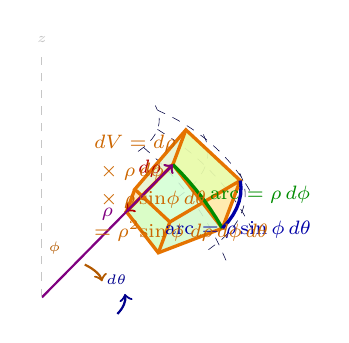
\begin{tikzpicture}[x={(0.85cm,-0.40cm)}, y={(0.85cm,0.40cm)}, z={(0cm,1.05cm)}, scale=1.6]
% Spherical dV element — drawn curved on the actual sphere surface,
% labeled to show WHY each side has length d_rho, rho*d_phi, rho*sin(phi)*d_theta.
% Parameters: rho in [1.0, 1.55], phi in [38, 58 deg], theta in [20, 50 deg]
\def\rI{1.0}  \def\rO{1.55}
\def\phA{38}  \def\phB{58}
\def\thA{20}  \def\thB{50}
\pgfmathsetmacro{\phM}{(\phA+\phB)/2}
\pgfmathsetmacro{\thM}{(\thA+\thB)/2}

% ---- Sphere shell context (partial wireframe, thin & dashed) ----
% A few latitude arcs in the phi range, front-facing
\foreach \ph in {30,45,60} {
  \pgfmathsetmacro{\rr}{\rO*sin(\ph)} \pgfmathsetmacro{\zz}{\rO*cos(\ph)}
  \draw[blue!25!black,very thin,dashed,domain=10:60,smooth,samples=8,variable=\t]
    plot ({\rr*cos(\t)},{\rr*sin(\t)},\zz);
}
% A few meridian arcs in the theta range
\foreach \th in {15,35,55} {
  \draw[blue!25!black,very thin,dashed,domain=30:65,smooth,samples=8,variable=\p]
    plot ({\rO*sin(\p)*cos(\th)},{\rO*sin(\p)*sin(\th)},{\rO*cos(\p)});
}

% ---- Faces of the curved dV element ----
% Inner face (rho=rI)
\fill[yellow!35,opacity=0.75]
  ({\rI*sin(\phA)*cos(\thA)},{\rI*sin(\phA)*sin(\thA)},{\rI*cos(\phA)})
  -- ({\rI*sin(\phB)*cos(\thA)},{\rI*sin(\phB)*sin(\thA)},{\rI*cos(\phB)})
  -- ({\rI*sin(\phB)*cos(\thB)},{\rI*sin(\phB)*sin(\thB)},{\rI*cos(\phB)})
  -- ({\rI*sin(\phA)*cos(\thB)},{\rI*sin(\phA)*sin(\thB)},{\rI*cos(\phA)}) -- cycle;
% Outer face (rho=rO)
\fill[yellow!60,opacity=0.85]
  ({\rO*sin(\phA)*cos(\thA)},{\rO*sin(\phA)*sin(\thA)},{\rO*cos(\phA)})
  -- ({\rO*sin(\phB)*cos(\thA)},{\rO*sin(\phB)*sin(\thA)},{\rO*cos(\phB)})
  -- ({\rO*sin(\phB)*cos(\thB)},{\rO*sin(\phB)*sin(\thB)},{\rO*cos(\phB)})
  -- ({\rO*sin(\phA)*cos(\thB)},{\rO*sin(\phA)*sin(\thB)},{\rO*cos(\phA)}) -- cycle;
% phi=phA face (top)
\fill[orange!25,opacity=0.70]
  ({\rI*sin(\phA)*cos(\thA)},{\rI*sin(\phA)*sin(\thA)},{\rI*cos(\phA)})
  -- ({\rO*sin(\phA)*cos(\thA)},{\rO*sin(\phA)*sin(\thA)},{\rO*cos(\phA)})
  -- ({\rO*sin(\phA)*cos(\thB)},{\rO*sin(\phA)*sin(\thB)},{\rO*cos(\phA)})
  -- ({\rI*sin(\phA)*cos(\thB)},{\rI*sin(\phA)*sin(\thB)},{\rI*cos(\phA)}) -- cycle;
% phi=phB face (bottom)
\fill[orange!20,opacity=0.65]
  ({\rI*sin(\phB)*cos(\thA)},{\rI*sin(\phB)*sin(\thA)},{\rI*cos(\phB)})
  -- ({\rO*sin(\phB)*cos(\thA)},{\rO*sin(\phB)*sin(\thA)},{\rO*cos(\phB)})
  -- ({\rO*sin(\phB)*cos(\thB)},{\rO*sin(\phB)*sin(\thB)},{\rO*cos(\phB)})
  -- ({\rI*sin(\phB)*cos(\thB)},{\rI*sin(\phB)*sin(\thB)},{\rI*cos(\phB)}) -- cycle;
% theta=thA face (front meridian)
\fill[green!20,opacity=0.72]
  ({\rI*sin(\phA)*cos(\thA)},{\rI*sin(\phA)*sin(\thA)},{\rI*cos(\phA)})
  -- ({\rI*sin(\phB)*cos(\thA)},{\rI*sin(\phB)*sin(\thA)},{\rI*cos(\phB)})
  -- ({\rO*sin(\phB)*cos(\thA)},{\rO*sin(\phB)*sin(\thA)},{\rO*cos(\phB)})
  -- ({\rO*sin(\phA)*cos(\thA)},{\rO*sin(\phA)*sin(\thA)},{\rO*cos(\phA)}) -- cycle;
% theta=thB face (back)
\fill[green!15,opacity=0.55]
  ({\rI*sin(\phA)*cos(\thB)},{\rI*sin(\phA)*sin(\thB)},{\rI*cos(\phA)})
  -- ({\rI*sin(\phB)*cos(\thB)},{\rI*sin(\phB)*sin(\thB)},{\rI*cos(\phB)})
  -- ({\rO*sin(\phB)*cos(\thB)},{\rO*sin(\phB)*sin(\thB)},{\rO*cos(\phB)})
  -- ({\rO*sin(\phA)*cos(\thB)},{\rO*sin(\phA)*sin(\thB)},{\rO*cos(\phA)}) -- cycle;

% ---- Edges of the curved dV element ----
\draw[orange!90!black,very thick]
  ({\rI*sin(\phA)*cos(\thA)},{\rI*sin(\phA)*sin(\thA)},{\rI*cos(\phA)})
  -- ({\rI*sin(\phB)*cos(\thA)},{\rI*sin(\phB)*sin(\thA)},{\rI*cos(\phB)})
  -- ({\rO*sin(\phB)*cos(\thA)},{\rO*sin(\phB)*sin(\thA)},{\rO*cos(\phB)})
  -- ({\rO*sin(\phA)*cos(\thA)},{\rO*sin(\phA)*sin(\thA)},{\rO*cos(\phA)}) -- cycle;
\draw[orange!90!black,very thick]
  ({\rI*sin(\phA)*cos(\thB)},{\rI*sin(\phA)*sin(\thB)},{\rI*cos(\phA)})
  -- ({\rI*sin(\phB)*cos(\thB)},{\rI*sin(\phB)*sin(\thB)},{\rI*cos(\phB)})
  -- ({\rO*sin(\phB)*cos(\thB)},{\rO*sin(\phB)*sin(\thB)},{\rO*cos(\phB)})
  -- ({\rO*sin(\phA)*cos(\thB)},{\rO*sin(\phA)*sin(\thB)},{\rO*cos(\phA)}) -- cycle;
\draw[orange!90!black,very thick]
  ({\rI*sin(\phA)*cos(\thA)},{\rI*sin(\phA)*sin(\thA)},{\rI*cos(\phA)})
  -- ({\rI*sin(\phA)*cos(\thB)},{\rI*sin(\phA)*sin(\thB)},{\rI*cos(\phA)});
\draw[orange!90!black,very thick]
  ({\rI*sin(\phB)*cos(\thA)},{\rI*sin(\phB)*sin(\thA)},{\rI*cos(\phB)})
  -- ({\rI*sin(\phB)*cos(\thB)},{\rI*sin(\phB)*sin(\thB)},{\rI*cos(\phB)});
\draw[orange!90!black,very thick]
  ({\rO*sin(\phA)*cos(\thA)},{\rO*sin(\phA)*sin(\thA)},{\rO*cos(\phA)})
  -- ({\rO*sin(\phA)*cos(\thB)},{\rO*sin(\phA)*sin(\thB)},{\rO*cos(\phA)});
\draw[orange!90!black,very thick]
  ({\rO*sin(\phB)*cos(\thA)},{\rO*sin(\phB)*sin(\thA)},{\rO*cos(\phB)})
  -- ({\rO*sin(\phB)*cos(\thB)},{\rO*sin(\phB)*sin(\thB)},{\rO*cos(\phB)});

% ---- d_rho label: radial edge on front-top corner ----
\draw[red!70!black,<->,thick]
  ({\rI*sin(\phA)*cos(\thA)},{\rI*sin(\phA)*sin(\thA)},{\rI*cos(\phA)})
  -- ({\rO*sin(\phA)*cos(\thA)},{\rO*sin(\phA)*sin(\thA)},{\rO*cos(\phA)})
  node[midway,above,font=\scriptsize,red!70!black]{$d\rho$};

% ---- rho*d_phi label: phi-arc on front face (theta=thA, rho=rO) ----
% Draw the actual arc along phi direction
\draw[green!55!black,very thick]
  plot[domain=\phA:\phB,samples=8,variable=\p]
    ({\rO*sin(\p)*cos(\thA)},{\rO*sin(\p)*sin(\thA)},{\rO*cos(\p)});
\pgfmathsetmacro{\labphx}{\rO*sin(\phM)*cos(\thA)}
\pgfmathsetmacro{\labphy}{\rO*sin(\phM)*sin(\thA)}
\pgfmathsetmacro{\labphz}{\rO*cos(\phM)}
\node[green!55!black,font=\scriptsize,right] at (\labphx,\labphy,\labphz)
  {arc $= \rho\,d\phi$};

% ---- rho*sin(phi)*d_theta label: theta-arc on outer-bottom face (phi=phB, rho=rO) ----
% The horizontal circle at phi=phB has radius rO*sin(phB)
\draw[blue!65!black,very thick]
  plot[domain=\thA:\thB,samples=8,variable=\t]
    ({\rO*sin(\phB)*cos(\t)},{\rO*sin(\phB)*sin(\t)},{\rO*cos(\phB)});
\pgfmathsetmacro{\labthx}{\rO*sin(\phB)*cos(\thM)}
\pgfmathsetmacro{\labthy}{\rO*sin(\phB)*sin(\thM)}
\pgfmathsetmacro{\labthz}{\rO*cos(\phB)}
\node[blue!65!black,font=\scriptsize,below] at (\labthx,\labthy,{\labthz-0.05})
  {arc $= \rho\sin\phi\,d\theta$};

% ---- rho vector from origin to near element ----
\draw[violet,thick,->] (0,0,0)
  -- ({\rO*sin(\phA)*cos(\thA)},{\rO*sin(\phA)*sin(\thA)},{\rO*cos(\phA)})
  node[midway,above,font=\scriptsize,violet]{$\rho$};

% ---- phi angle arc (in meridian plane for thA edge) ----
% Draw arc from z-axis down to phi=phA
\draw[orange!70!black,thick,->]
  ({0.4*cos(0)},{0.4*sin(0)},{\rO*0.4/\rO})
  arc[start angle=90,delta angle={-\phA},radius=0.4];
\node[orange!70!black,font=\tiny] at ({0.28*sin(\phA/2)*cos(\thA)},{0.28*sin(\phA/2)*sin(\thA)},{0.42*cos(\phA/2)}) {$\phi$};

% ---- theta angle arc (on equatorial plane, inner ring) ----
\draw[blue!55!black,thick,->]
  ({0.55*cos(\thA)},{0.55*sin(\thA)},0) arc[start angle=\thA,end angle=\thB,radius=0.55];
\node[blue!55!black,font=\tiny] at ({0.5*cos(\thM)},{0.5*sin(\thM)},0.18) {$d\theta$};

% Dashed z-axis reference
\draw[gray!45,dashed,thin] (0,0,0) -- (0,0,{\rO+0.3}) node[above,font=\tiny,gray!45]{$z$};

% ---- dV formula annotation ----
\node[font=\scriptsize,align=left,orange!80!black] at (1.8,-0.5,1.7) {
  $dV = d\rho$\\[2pt]
  $\;\times\;\rho\,d\phi$\\[2pt]
  $\;\times\;\rho\sin\!\phi\,d\theta$\\[4pt]
  $= \rho^2\!\sin\phi\;d\rho\,d\phi\,d\theta$
};

\end{tikzpicture}
\end{center}

\textbf{The three physical edge lengths} of the infinitesimal spherical box are: a purely radial step $d\rho$; a meridional arc of length $\rho\,d\phi$ (sweeping angle $d\phi$ along a circle of radius $\rho$); and an azimuthal arc of length $\rho\sin\phi\,d\theta$ (sweeping angle $d\theta$ along the horizontal circle at colatitude $\phi$, which has radius $\rho\sin\phi$ --- shrinking to zero at the poles where $\sin\phi=0$).  Linearizing and multiplying gives $dV = \rho^2\sin\phi\,d\rho\,d\phi\,d\theta$.

\begin{problem}
The spherical volume element $dV = \rho^2\sin\phi\,d\rho\,d\phi\,d\theta$ has:

An extra factor of $\rho^2$: \wordChoice{\choice[correct]{Yes}\choice{No}}

An extra factor of $\sin\phi$: \wordChoice{\choice[correct]{Yes}\choice{No}}

These factors account for:
\begin{multipleChoice}
    \choice{Mathematical complexity}
    \choice[correct]{The geometry of spherical shells and how they expand with radius}
    \choice{Random constants}
\end{multipleChoice}

\begin{feedback}
The $\rho^2\sin\phi$ factor is crucial! It accounts for how spherical volume elements grow with radius and latitude.
\end{feedback}
\end{problem}

\begin{problem}
Explore spherical coordinates visually.

\begin{expandable}{stuff}{GeoGebra Instructions}
    Select ``Show Sphere'' view. Use sliders for $\rho$, $\phi$, $\theta$. Zoom to see the volume element shape—it's like a tiny curved box on a sphere!
\end{expandable}

\begin{center}
\geogebra{xqrs44yg}{750}{675}
\end{center}

In spherical coordinates:
\begin{selectAll}
    \choice[correct]{$\rho$ measures distance from origin}
    \choice[correct]{$\phi$ measures angle from the positive $z$-axis (colatitude)}
    \choice[correct]{$\theta$ measures rotation around $z$-axis (azimuth)}
    \choice{All angles range from $0$ to $2\pi$}
\end{selectAll}

Typical ranges are:
\begin{itemize}
    \item $\rho \geq 0$
    \item $0 \leq \phi \leq \answer{\pi}$ (from north pole to south pole)
    \item $0 \leq \theta \leq \answer{2\pi}$ (full rotation)
\end{itemize}

\begin{feedback}
Spherical coordinates are perfect for spheres, cones, and any geometry with radial symmetry!
\end{feedback}
\end{problem}

Before going into the final example, watch this video for a visual explanation of the spherical integration:


\youtube{sAEEWP6FBXA}


\begin{problem}
Find the mass of a sphere of radius $R$ with variable density $\delta(\rho) = k\rho$ (the fluid is denser farther from the center).

\begin{center}
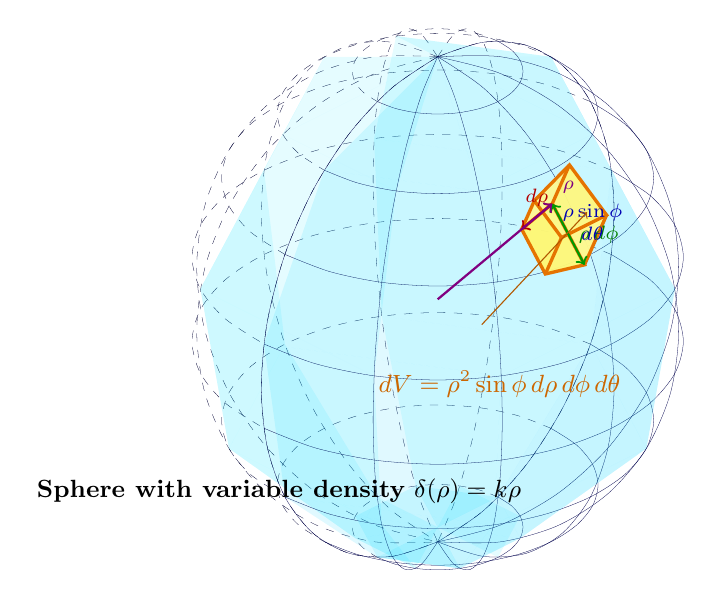
\begin{tikzpicture}[x={(0.8cm,-0.4cm)}, y={(0.8cm,0.4cm)}, z={(0cm,1.1cm)}, scale=1.4]
% Sphere wireframe + one highlighted dV wedge element — no axes, minimal wireframe
\def\RS{2.0}

% --- Back hemisphere wireframe (thin dashed — more lines for rounder look) ---
\foreach \ph in {20,40,60,80,100,120,140,160} {
  \pgfmathsetmacro{\rr}{\RS*sin(\ph)}
  \pgfmathsetmacro{\zz}{\RS*cos(\ph)}
  \draw[blue!20!black,ultra thin,dashed,domain=90:270,smooth,samples=13,variable=\t]
    plot ({\rr*cos(\t)},{\rr*sin(\t)},\zz);
}
\foreach \th in {90,120,150,180,210,240,270} {
  \draw[blue!20!black,ultra thin,dashed,domain=0:180,smooth,samples=13,variable=\p]
    plot ({\RS*sin(\p)*cos(\th)},{\RS*sin(\p)*sin(\th)},{\RS*cos(\p)});
}

% Light fill on back hemisphere (very faint)
\foreach \ph in {0,40,...,160} {
  \pgfmathsetmacro{\phn}{\ph+40}
  \pgfmathsetmacro{\ra}{\RS*sin(\ph)} \pgfmathsetmacro{\za}{\RS*cos(\ph)}
  \pgfmathsetmacro{\rb}{\RS*sin(\phn)} \pgfmathsetmacro{\zb}{\RS*cos(\phn)}
  \foreach \th in {90,180,240} {
    \pgfmathsetmacro{\thn}{\th+60}
    \fill[blue!12!cyan,opacity=0.10]
      ({\ra*cos(\th)},{\ra*sin(\th)},\za)
      -- ({\rb*cos(\th)},{\rb*sin(\th)},\zb)
      -- ({\rb*cos(\thn)},{\rb*sin(\thn)},\zb)
      -- ({\ra*cos(\thn)},{\ra*sin(\thn)},\za) -- cycle;
  }
}

% --- Front hemisphere (thin lines only — more lines for rounder look) ---
\foreach \ph in {20,40,60,80,100,120,140,160} {
  \pgfmathsetmacro{\rr}{\RS*sin(\ph)}
  \pgfmathsetmacro{\zz}{\RS*cos(\ph)}
  \draw[blue!30!black,ultra thin,domain=-90:90,smooth,samples=13,variable=\t]
    plot ({\rr*cos(\t)},{\rr*sin(\t)},\zz);
}
\foreach \th in {-90,-60,-30,0,30,60,90} {
  \draw[blue!30!black,ultra thin,domain=0:180,smooth,samples=13,variable=\p]
    plot ({\RS*sin(\p)*cos(\th)},{\RS*sin(\p)*sin(\th)},{\RS*cos(\p)});
}

% Light fill on front hemisphere (gentle)
\foreach \ph in {0,40,...,160} {
  \pgfmathsetmacro{\phn}{\ph+40}
  \pgfmathsetmacro{\ra}{\RS*sin(\ph)} \pgfmathsetmacro{\za}{\RS*cos(\ph)}
  \pgfmathsetmacro{\rb}{\RS*sin(\phn)} \pgfmathsetmacro{\zb}{\RS*cos(\phn)}
  \foreach \th in {-90,-30,...,60} {
    \pgfmathsetmacro{\thn}{\th+60}
    \fill[blue!18!cyan,opacity=0.12]
      ({\ra*cos(\th)},{\ra*sin(\th)},\za)
      -- ({\rb*cos(\th)},{\rb*sin(\th)},\zb)
      -- ({\rb*cos(\thn)},{\rb*sin(\thn)},\zb)
      -- ({\ra*cos(\thn)},{\ra*sin(\thn)},\za) -- cycle;
  }
}

% --- Highlighted dV wedge element ---
% rho in [1.1,1.5], phi in [45,65 deg], theta in [15,50 deg]
\def\rI{1.1} \def\rO{1.5}
\def\phA{45} \def\phB{65}
\def\thA{15} \def\thB{50}

% 8 corner coordinates (pre-compute with helper macros)
% inner/outer, phi low/high, theta low/high: notation (rho, ph, th)
% We draw 6 faces as quads

% Face 1: inner sphere face (rho=rI, phi, theta sweep)
\fill[yellow!50,opacity=0.80]
  ({\rI*sin(\phA)*cos(\thA)},{\rI*sin(\phA)*sin(\thA)},{\rI*cos(\phA)})
  -- ({\rI*sin(\phB)*cos(\thA)},{\rI*sin(\phB)*sin(\thA)},{\rI*cos(\phB)})
  -- ({\rI*sin(\phB)*cos(\thB)},{\rI*sin(\phB)*sin(\thB)},{\rI*cos(\phB)})
  -- ({\rI*sin(\phA)*cos(\thB)},{\rI*sin(\phA)*sin(\thB)},{\rI*cos(\phA)}) -- cycle;

% Face 2: outer sphere face (rho=rO)
\fill[yellow!60,opacity=0.85]
  ({\rO*sin(\phA)*cos(\thA)},{\rO*sin(\phA)*sin(\thA)},{\rO*cos(\phA)})
  -- ({\rO*sin(\phB)*cos(\thA)},{\rO*sin(\phB)*sin(\thA)},{\rO*cos(\phB)})
  -- ({\rO*sin(\phB)*cos(\thB)},{\rO*sin(\phB)*sin(\thB)},{\rO*cos(\phB)})
  -- ({\rO*sin(\phA)*cos(\thB)},{\rO*sin(\phA)*sin(\thB)},{\rO*cos(\phA)}) -- cycle;

% Face 3: phi=phA (upper cone face)
\fill[yellow!40,opacity=0.75]
  ({\rI*sin(\phA)*cos(\thA)},{\rI*sin(\phA)*sin(\thA)},{\rI*cos(\phA)})
  -- ({\rO*sin(\phA)*cos(\thA)},{\rO*sin(\phA)*sin(\thA)},{\rO*cos(\phA)})
  -- ({\rO*sin(\phA)*cos(\thB)},{\rO*sin(\phA)*sin(\thB)},{\rO*cos(\phA)})
  -- ({\rI*sin(\phA)*cos(\thB)},{\rI*sin(\phA)*sin(\thB)},{\rI*cos(\phA)}) -- cycle;

% Face 4: phi=phB (lower cone face)
\fill[yellow!40,opacity=0.75]
  ({\rI*sin(\phB)*cos(\thA)},{\rI*sin(\phB)*sin(\thA)},{\rI*cos(\phB)})
  -- ({\rO*sin(\phB)*cos(\thA)},{\rO*sin(\phB)*sin(\thA)},{\rO*cos(\phB)})
  -- ({\rO*sin(\phB)*cos(\thB)},{\rO*sin(\phB)*sin(\thB)},{\rO*cos(\phB)})
  -- ({\rI*sin(\phB)*cos(\thB)},{\rI*sin(\phB)*sin(\thB)},{\rI*cos(\phB)}) -- cycle;

% Face 5: theta=thA (front meridian face)
\fill[yellow!55,opacity=0.82]
  ({\rI*sin(\phA)*cos(\thA)},{\rI*sin(\phA)*sin(\thA)},{\rI*cos(\phA)})
  -- ({\rI*sin(\phB)*cos(\thA)},{\rI*sin(\phB)*sin(\thA)},{\rI*cos(\phB)})
  -- ({\rO*sin(\phB)*cos(\thA)},{\rO*sin(\phB)*sin(\thA)},{\rO*cos(\phB)})
  -- ({\rO*sin(\phA)*cos(\thA)},{\rO*sin(\phA)*sin(\thA)},{\rO*cos(\phA)}) -- cycle;

% Face 6: theta=thB (back face of wedge -- draw at lower opacity)
\fill[yellow!45,opacity=0.65]
  ({\rI*sin(\phA)*cos(\thB)},{\rI*sin(\phA)*sin(\thB)},{\rI*cos(\phA)})
  -- ({\rI*sin(\phB)*cos(\thB)},{\rI*sin(\phB)*sin(\thB)},{\rI*cos(\phB)})
  -- ({\rO*sin(\phB)*cos(\thB)},{\rO*sin(\phB)*sin(\thB)},{\rO*cos(\phB)})
  -- ({\rO*sin(\phA)*cos(\thB)},{\rO*sin(\phA)*sin(\thB)},{\rO*cos(\phA)}) -- cycle;

% Draw wedge edges
\draw[orange!90!black,very thick]
  ({\rI*sin(\phA)*cos(\thA)},{\rI*sin(\phA)*sin(\thA)},{\rI*cos(\phA)})
  -- ({\rI*sin(\phB)*cos(\thA)},{\rI*sin(\phB)*sin(\thA)},{\rI*cos(\phB)})
  -- ({\rO*sin(\phB)*cos(\thA)},{\rO*sin(\phB)*sin(\thA)},{\rO*cos(\phB)})
  -- ({\rO*sin(\phA)*cos(\thA)},{\rO*sin(\phA)*sin(\thA)},{\rO*cos(\phA)}) -- cycle;
\draw[orange!90!black,very thick]
  ({\rI*sin(\phA)*cos(\thB)},{\rI*sin(\phA)*sin(\thB)},{\rI*cos(\phA)})
  -- ({\rI*sin(\phB)*cos(\thB)},{\rI*sin(\phB)*sin(\thB)},{\rI*cos(\phB)})
  -- ({\rO*sin(\phB)*cos(\thB)},{\rO*sin(\phB)*sin(\thB)},{\rO*cos(\phB)})
  -- ({\rO*sin(\phA)*cos(\thB)},{\rO*sin(\phA)*sin(\thB)},{\rO*cos(\phA)}) -- cycle;
\draw[orange!90!black,very thick]
  ({\rI*sin(\phA)*cos(\thA)},{\rI*sin(\phA)*sin(\thA)},{\rI*cos(\phA)})
  -- ({\rI*sin(\phA)*cos(\thB)},{\rI*sin(\phA)*sin(\thB)},{\rI*cos(\phA)});
\draw[orange!90!black,very thick]
  ({\rI*sin(\phB)*cos(\thA)},{\rI*sin(\phB)*sin(\thA)},{\rI*cos(\phB)})
  -- ({\rI*sin(\phB)*cos(\thB)},{\rI*sin(\phB)*sin(\thB)},{\rI*cos(\phB)});
\draw[orange!90!black,very thick]
  ({\rO*sin(\phA)*cos(\thA)},{\rO*sin(\phA)*sin(\thA)},{\rO*cos(\phA)})
  -- ({\rO*sin(\phA)*cos(\thB)},{\rO*sin(\phA)*sin(\thB)},{\rO*cos(\phA)});
\draw[orange!90!black,very thick]
  ({\rO*sin(\phB)*cos(\thA)},{\rO*sin(\phB)*sin(\thA)},{\rO*cos(\phB)})
  -- ({\rO*sin(\phB)*cos(\thB)},{\rO*sin(\phB)*sin(\thB)},{\rO*cos(\phB)});

% Labels: edge dimensions on front face
\draw[red!70!black,<->,thick]
  ({\rI*sin(\phA)*cos(\thA)},{\rI*sin(\phA)*sin(\thA)},{\rI*cos(\phA)})
  -- ({\rO*sin(\phA)*cos(\thA)},{\rO*sin(\phA)*sin(\thA)},{\rO*cos(\phA)})
  node[midway,above,font=\scriptsize,red!70!black]{$d\rho$};

\draw[green!60!black,<->,thick]
  ({\rO*sin(\phA)*cos(\thA)},{\rO*sin(\phA)*sin(\thA)},{\rO*cos(\phA)})
  -- ({\rO*sin(\phB)*cos(\thA)},{\rO*sin(\phB)*sin(\thA)},{\rO*cos(\phB)})
  node[midway,right,font=\scriptsize,green!50!black]{$\rho\,d\phi$};

% theta arc label
\node[font=\scriptsize,blue!70!black,align=center] at
  ({(\rO+0.25)*sin(55)*cos(\thA)},{(\rO+0.25)*sin(55)*sin(\thA)},{(\rO+0.25)*cos(55)})
  {$\rho\sin\phi$\\$d\theta$};

% dV label
\node[font=\small,orange!80!black,align=center] at (2.0,-1.3,0.5)
  {$dV = \rho^2\sin\phi\,d\rho\,d\phi\,d\theta$};
\draw[orange!70!black,->,thin]
  (1.5,-1.0,0.7) -- ({\rO*sin(55)*cos(32)},{\rO*sin(55)*sin(32)},{\rO*cos(55)});

% rho vector to P
\draw[violet,thick,->] (0,0,0) -- ({\rO*sin(\phA)*cos(\thA)},{\rO*sin(\phA)*sin(\thA)},{\rO*cos(\phA)})
  node[above right,font=\scriptsize,violet]{$\rho$};

\node[font=\small,align=center,below] at (0.2,-2.0,-0.6)
  {\textbf{Sphere with variable density} $\delta(\rho)=k\rho$};
\end{tikzpicture}
\end{center}

In spherical coordinates, the sphere is simply: $0 \leq \rho \leq \answer{R}$

Full angular coverage: $0 \leq \phi \leq \answer{\pi}$, $0 \leq \theta \leq \answer{2\pi}$

The mass element is $dM = \delta(\rho)\,dV = k\rho \cdot \rho^2\sin\phi\,d\rho\,d\phi\,d\theta = k\rho^3\sin\phi\,d\rho\,d\phi\,d\theta$.

$$M = \int_0^{2\pi}\int_0^{\pi}\int_0^R k\rho^3\sin\phi\,d\rho\,d\phi\,d\theta$$

\textbf{Inner integral (w.r.t. $\rho$):}
$$\int_0^R k\rho^3\,d\rho = \left[\frac{k\rho^4}{4}\right]_0^R = \answer{kR^4/4}$$

\textbf{Middle integral (w.r.t. $\phi$):}
$$\int_0^{\pi} \frac{kR^4}{4}\sin\phi\,d\phi = \frac{kR^4}{4}[-\cos\phi]_0^{\pi} = \frac{kR^4}{4}[1-(-1)] = \answer{kR^4/2}$$

\textbf{Outer integral (w.r.t. $\theta$):}
$$\int_0^{2\pi} \frac{kR^4}{2}\,d\theta = \frac{kR^4}{2} \cdot 2\pi = \answer{k\pi R^4}$$

So the total mass is $M = k\pi R^4$.

Notice: if you set $k=0$ (uniform zero density), $M=0$. If you use $\delta=k$ (constant density), the standard volume formula gives $V = \frac{4}{3}\pi R^3$, and $M = kV = \frac{4k\pi R^3}{3}$. The variable density $\delta=k\rho$ shifts mass toward the outer shell.

\begin{feedback}
Spherical coordinates turned what would have been a nightmare integral (with $\sqrt{x^2+y^2+z^2}$ in the density) into a clean separable integral with constant bounds! The 3D wedge diagram shows the three physical edge lengths: $d\rho$, $\rho\,d\phi$, and $\rho\sin\phi\,d\theta$, whose product gives the volume element $\rho^2\sin\phi\,d\rho\,d\phi\,d\theta$.
\end{feedback}
\end{problem}


\end{document}
